\documentclass[a4paper,12pt]{report}
\usepackage[utf8]{inputenc}
\usepackage{graphicx}
\usepackage{hyperref}

\graphicspath{ {./images/} }

\begin{document}
\title{UNIBOssfight}
\author{Livia Cardaccia, Denise Nanni, Giovanni Prete, Matteo Sartini}
\date{January 2023}
\maketitle
\newpage
\large
\tableofcontents
\newpage

\chapter{Analisi}

\section{Requisiti}
Il team si pone come obiettivo quello di realizzare una versione personalizzata del noto gioco arcade Metal Slug, ambientato nella nostra università.
Lo scopo del gioco è quello di conseguire la laurea superando gli esami, rappresentati da una serie di livelli platform, ossia in cui la meccanica di gioco implica principalmente l'attraversamento di livelli costituiti da piattaforme, spesso disposte su più piani.
In ogni livello sono presenti diversi minions che ostacolano la corsa del giocatore, e un boss finale, rappresentato dal docente del corso, la cui sconfitta determinerà il superamento dell'esame.
\subsection{Requisiti funzionali}
\begin{itemize}
\item Menù principale che permette all'utente di scegliere il livello di gioco, consultare i comandi, iniziare una nuova partita e uscire dal gioco.
\item Gestione dell'input simultaneo per il movimento e la gestione dell'arma.
\item Movimento di base dei nemici.
\item Implementazione di un'arma a fuoco automatico che verrà puntata in base alla posizione del mouse.
\item Calcolo del voto finale basato nemici sconfitti
e monete CFU raccolte.
\end{itemize}
\subsection{Requisiti non funzionali}
\begin{itemize}
\item Il gioco dovrà risultare fluido, con un frame rate minimo di 30 FPS.
\item Il gioco avrà una bassa latenza di input
\end{itemize}
\newpage
\section{Analisi e modello del dominio}
Il giocatore dovrà superare una serie di livelli in cui incontrerà due tipologie di ostacoli: nemici in movimento, che possono provocargli danno, e ostacoli di tipo ambientale.
Il giocatore potrà affrontare i nemici con l'arma in dotazione, stando attento a non esaurire la vita a sua disposizione, o scegliere di evitarli quando possibile (pena decurtazione del punteggio).
Gli ostacoli ambientali invece consisteranno in muri da scavalcare, fiamme e spine da evitare.
Alla fine del livello il personaggio si troverà ad affrontare un boss finale che disporrà di una quantità superiore di punti vita e arrecherà più danno rispetto ai nemici comuni.
Si denoteranno due categorie principali di entità, quelle passive come gli ostacoli, e quelle attive, come il giocatore e i nemici, che si muoveranno nel mondo e interagiranno in diversi modi con esso. Una delle difficoltà principali sarà quella di identificare questi oggetti e di gestire le interazioni che essi avranno tra loro.

\begin{figure}[ht]
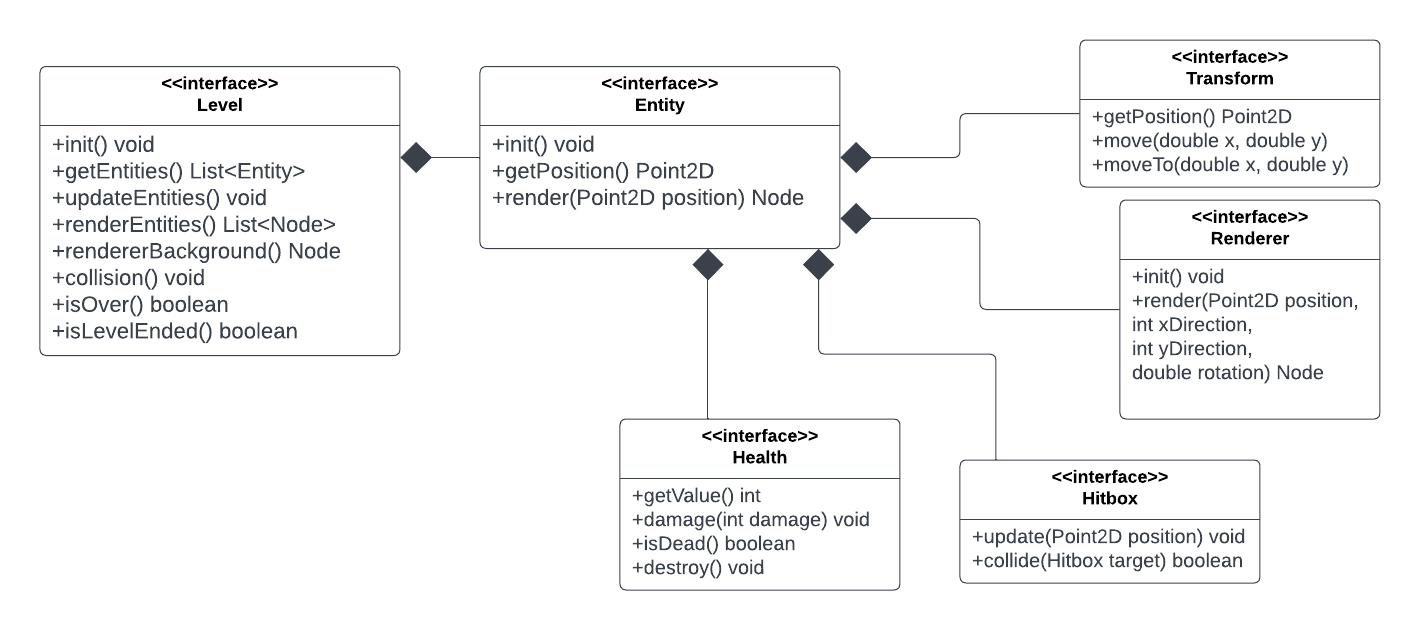
\includegraphics[width=0.8\textwidth]{umlModello.png}
\caption{Modello del dominio}
\label{fig:schgen}
\end{figure}


\chapter{Design}
\section{Architettura}
Questo progetto è stato sviluppato attraverso il pattern architetturale ECS, Entity Component System.
In ECS, le Entity sono tutte le entità di gioco, ovvero degli oggetti general purpose, che si compongono dei Components; questi ultimi modellano una determinata caratteristica di un'entità e mantengono i dati relativi ad essa. Il System è tutto ciò che modifica le entità, agendo sui loro componenti. Nella nostra applicazione le entity sono tutti gli attori del mondo di gioco, ad esempio il giocatore e i nemici, decorati da componenti che modellano il concetto di movimento e posizione con il Transform, le collisioni con il Collider, il comportamento con il Behaviour e simili, i quali vengono gestiti dal Level che rappresenta il sistema.
Nonostante non avessimo affrontato a lezione il pattern ECS, lo abbiamo scelto perché ci sembrava adatto ad un progetto come il nostro, dato che viene ampiamente utilizzato nello sviluppo di videogiochi, è versatile e facilmente estendibile.
L'aspetto caratteristico di ECS è che ogni entità si autogestisce, sia per quanto riguarda aspetti come il movimento, sia per altri aspetti come la renderizzazione; per tale motivo, utilizzando questo pattern potrebbe risultare poco agevole sostituire in blocco la view, tuttavia può essere fatto effettuando delle modifiche minori, in particolare al component Renderer.

\begin{figure}[ht]
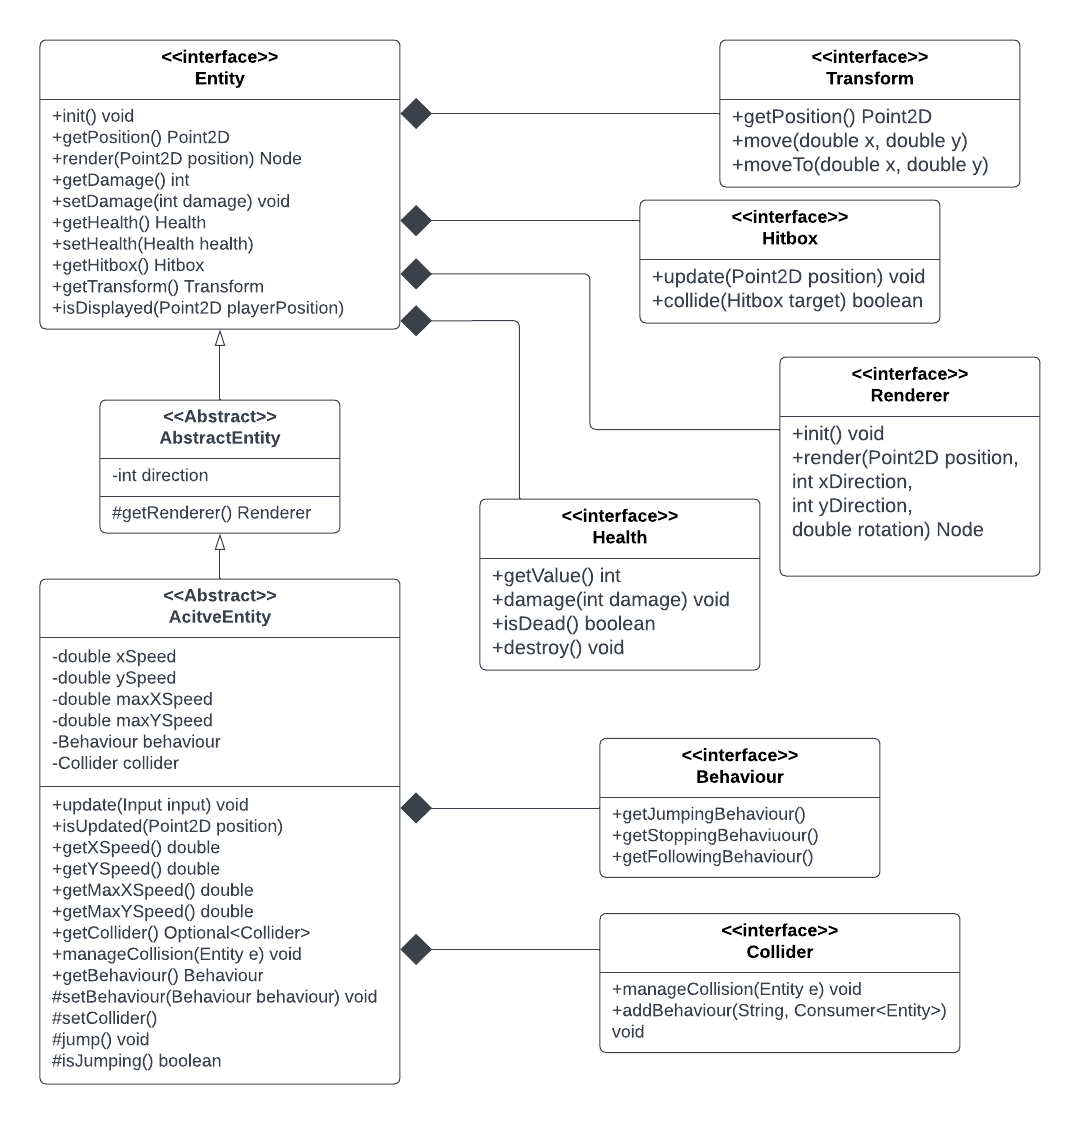
\includegraphics[width=1\textwidth]{umlEntityComponents.png}
\caption{Entità attive}
\label{fig:schgen}
\end{figure}

\newpage
\section{Design dettagliato}
Di seguito lo schema generale delle entità attive.
\begin{figure}[ht]
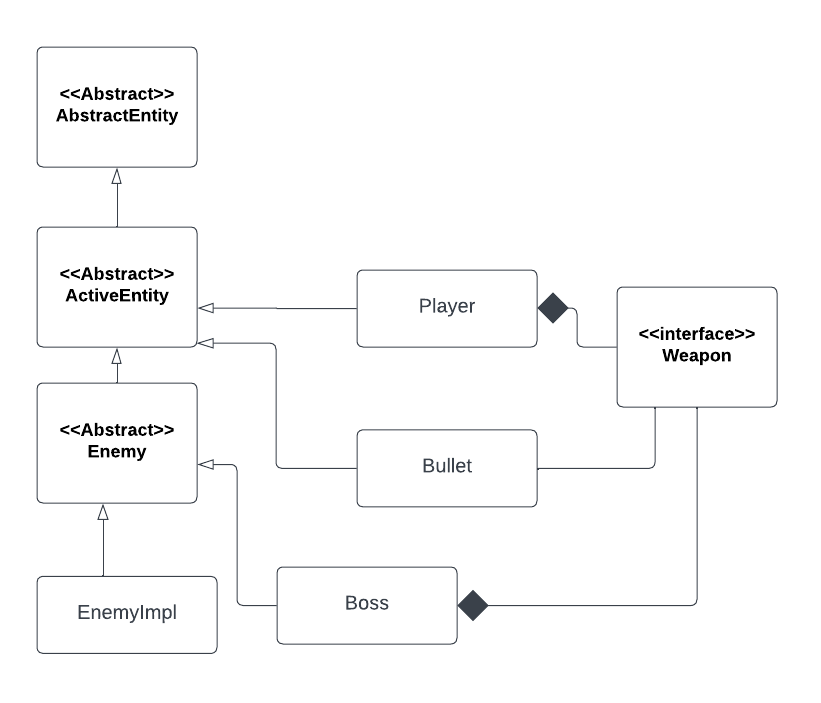
\includegraphics[width=1\textwidth]{umlAttive.png}
\caption{UML delle entità attive}
\label{fig:schgen}
\end{figure}
\subsection{Livia Cardaccia}
\textbf{Behaviour}\\
\\
Già in fase di analisi, abbiamo ritenuto necessario che le entità del nostro gioco potessero avere dei comportamenti specifici, come ad esempio la necessità di fermarsi di fronte ad un ostacolo come un muro o quella di saltare su un ostacolo come una piattaforma.
Nell'ottica ECS, è sembrato lineare racchiudere questi comportamenti in un Component, chiamato appunto Behaviour.\\ Dato che le varie entità in movimento, quali nemici, boss e giocatore, possono assumere comportamenti diversi, rendendo quindi necessaria la possibilità di suddividere le fasi di creazione del component, per implementare il Behaviour mi è sembrato conveniente sfruttare un pattern visto a lezione, il Builder.\\ Entrando nello specifico, ho scritto un'interfaccia Behaviour con metodi setter e getter, utilizzati poi per l'implementazione del component e per richiamarlo ove necesssario nel codice.\\
Nell'interfaccia BehaviourBuilder ci sono invece i metodi per poter aggiungere comportamenti, implementati poi attraverso \texttt{BiConsumer} e\\ \texttt{BiFunction} e che usano al loro interno altri component delle entità, come ad esempio il Transform e la Hitbox: attualmente vi sono cinque comportamenti, per saltare sulle Platform, per essere fermati di lato e dal basso da un Wall, per seguire e per volare sopra al player.\\
Il grande punto di forza di questo pattern è che rimane sempre aperta la possibilità di aggiungere nuovi comportamenti con facilità, il che rende il Behaviour un component flessibile ed estendibile.

\begin{figure}[ht]
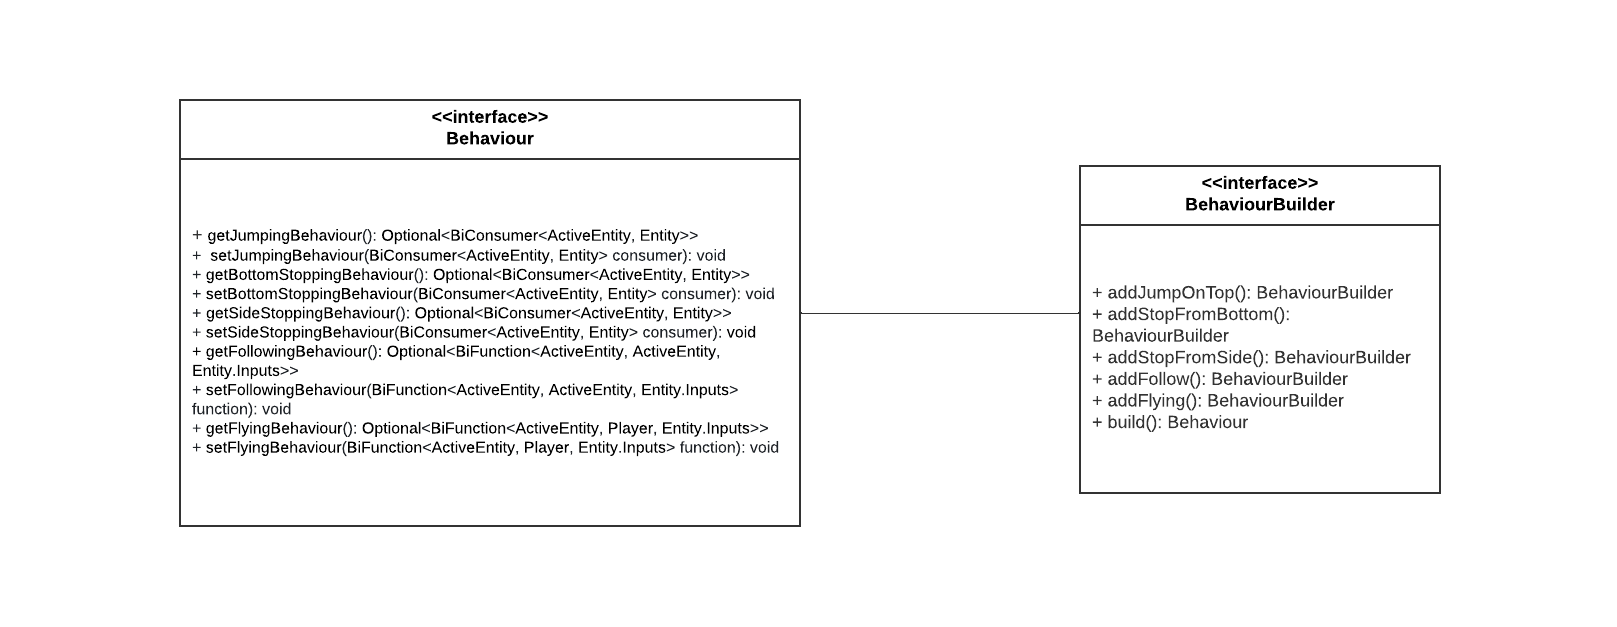
\includegraphics[width=1\textwidth]{umlBehaviour.png}
\caption{UML del component Behaviour}
\label{fig:schgen}
\end{figure}

\newpage
\textbf{Ostacoli}\\
\\
Gli ostacoli del nostro gioco, di cui mi sono occupata, sono di due tipi, quelli che causano e quelli che non causano danno al giocatore. I secondi, ovvero Platform e Wall, hanno delle funzioni che controllano se è avvenuta una collisione con le entità del gioco in movimento e sfruttano il Behaviour di queste per, in un caso, permettere all'entità di saltare su di essi, nell'altro per fermare la corsa dell'entità.\\
Ci sono inoltre i Coin, che non arrecano danno ma costituiscono un'aggiunta di punti per il giocatore, vanno quindi ad aumentare il voto finale di quest'ultimo.\\

\begin{figure}[ht]
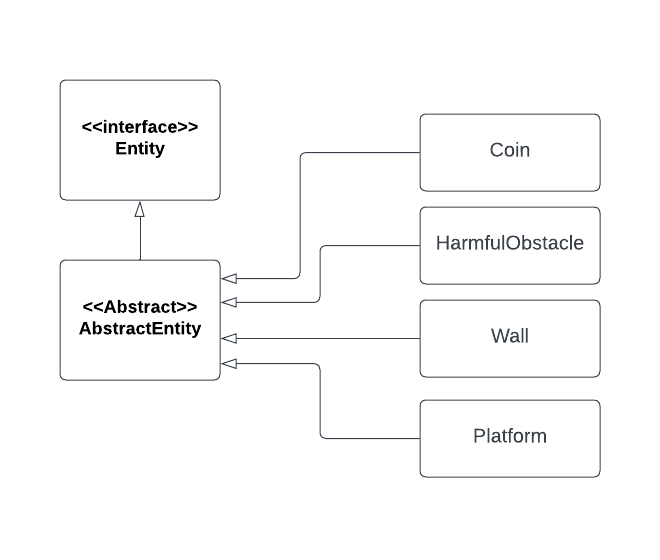
\includegraphics[width=1\textwidth]{umlObstacles.png}
\caption{UML degli ostacoli del gioco}
\label{fig:schgen}
\end{figure}

\newpage
\textbf{Menu principale e SecondaryStage}\\
\\
Durante lo sviluppo del software, un mio compito è stato anche quello di progettare ed implementare il menu di gioco con i vari bottoni e le relative sub scenes: per fare ciò, ho largamente utilizzato la libreria JavaFX.\\
Nel menu, è il ViewManager che si occupa di settare l'appearence generale e mette a disposizione dei metodi per aggiungere immagini e background, che ho richiamato nel Game.
Inoltre, sempre nel Game, ho gestito il cambio di stage, in particolare a fine partita viene data la possibilità all'utente di proseguire con il livello successivo, in caso di vittoria, o di ricominciare la partita in caso di sconfitta; in entrambi i casi è presente un pulsante per tornare alla home.\\
Per fare questo ho utilizzato una classe innestata, SecondaryStage, nel quale sfrutto sia metodi della libreria JavaFX sia metodi scritti da me nel ViewManager.

\subsection{Denise Nanni}
\textbf{Collisioni}\\
\\
La mia parte di progetto consisteva principalmente nella gestione delle collisioni tra le varie entità.
Per un gioco di questo tipo, è di fondamentale importanza distinguere i vari tipi di collisione e le direzioni da cui esse avvengono. Si è reso necessario avere un meccanismo che riconoscesse l'entità con cui è avvenuta la collisione e la gestisse secondo un comportamento ad hoc per tale entità.

\begin{figure}[ht]
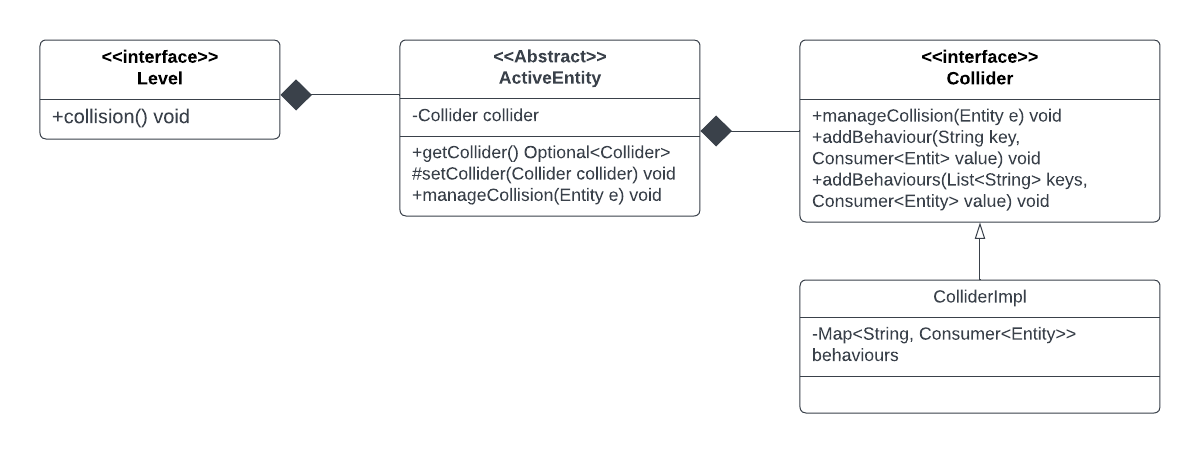
\includegraphics[width=1\textwidth]{umlCollider.png}
\caption{UML del Collider}
\label{fig:schgen}
\end{figure}

La gestione viene effettuata dalle entità attive che rispondono al contatto modificando il proprio stato, ad esempio il giocatore che collide con un nemico modifica il suo stato per essere respinto e per infliggersi il danno ricevuto.
Si è posto il problema di come distingere i vari attori, visto che per ciasciuno di essi vi era un'operazione specifica da eseguire. Inizialmente, la scelta è ricaduta erroneamente sull'utilizzo di un enumerazione attraverso la quale si verificava il tipo di istanza attraverso la reflection. Tuttavia, tale soluzione rendeva il software meno flessibile ad eventuali estensioni come aggiunta di nuovi tipi di entità.
La scelta finale è stata quella di utilizzare delle semplici stringhe in modo tale da poter aggiungere facilmente nuovi tipi. Ad ogni tipo è associata una funzione \texttt{Consumer} che prende in input l'entità con cui si è colliso e nella quale vengono svolte le operazioni specifiche in reazione a quella determinata collisione.\\
Sempre in relazione alla rilevazione delle collisioni, è stato necessario distinguere le varie direzioni per poter associare il relativo comportamento; ad esempio, un muro ferma l'entità attiva da tutte le direzioni, però se la collisione è avvenuta dai lati, deve semplicemente bloccare l'avanzamento, mentre se è avvenuta da sopra, deve far si che l'entità vi cammini sopra, e così via.
A questo scopo, si era pensato di utilizzare la posizione precedente dell'entità, poi ho optato per una rilevazione più superficiale, ma comunque abbastanza funzionale, basata sulla dimensione dell'intersezione della collisione.\\
\\
\textbf{Logger}\\
\\
Durante lo sviluppo, si è resa necessaria una funzionalità che permettesse di mantenere uno storico degli errori verificatisi durante l'esecuzione. Ho quindi utilizzato il pattern creazionale Singleton per realizzare un logger \texttt{AppLogger} che estende il logger di default di Java, in modo da avere un'unica istanza per tutto l'applicativo che scrivesse su un singolo file di log.
\newpage
\subsection{Giovanni Prete}
\textbf{Renderer}\\
\\
Il mio ruolo principale all'interno del progetto è stata la realizzazione del Renderer component e di tutte le sue declinazioni.
Questo component ha il compito di rappresentare su schermo le Entity di gioco e, per farlo ho sfruttato le potenzialità degli elementi della libreria di javaFX.

\begin{figure}[ht]
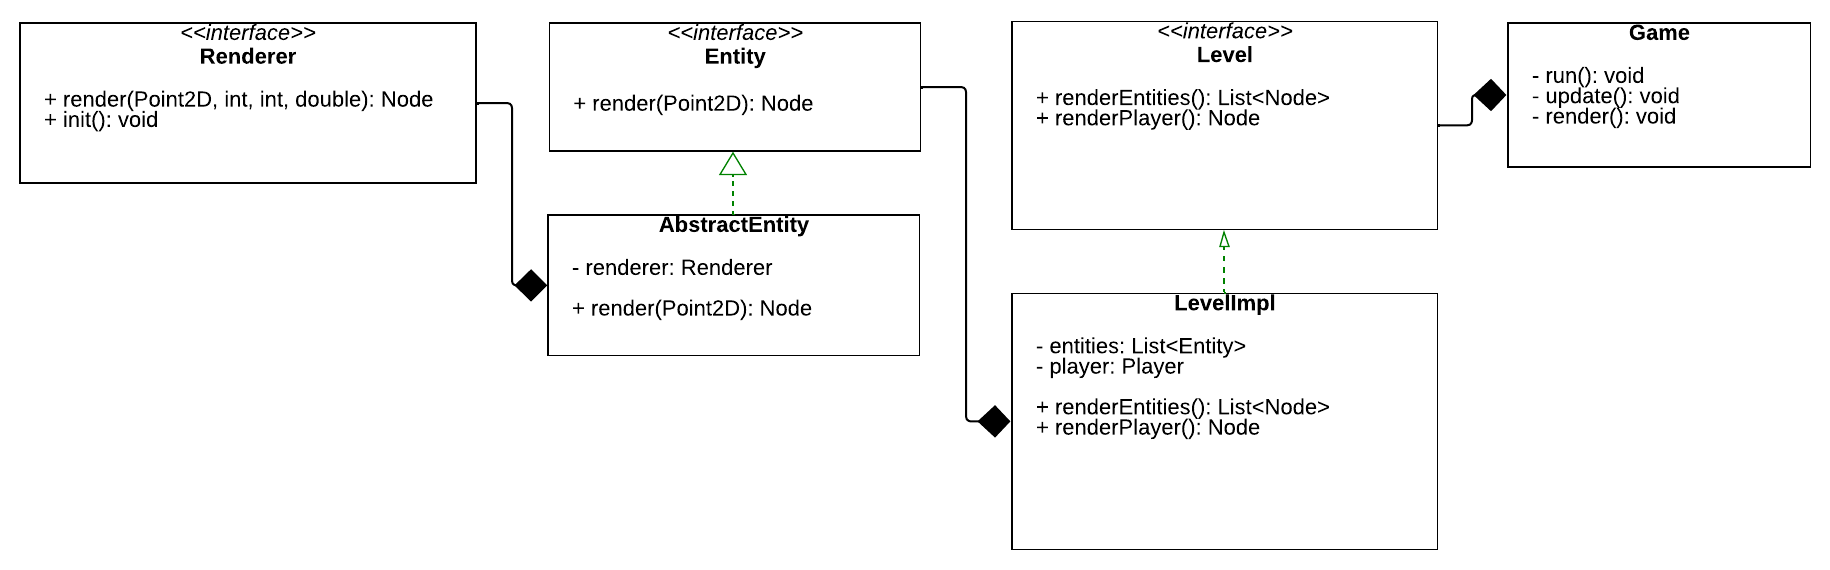
\includegraphics[width=1\textwidth]{images/renderer.png}
\caption{Integrazione del Renderer}
\label{fig:renderer}
\end{figure}

Le due funzioni principali del component sono init e render.
La prima inizializza l'oggetto in modo diverso a seconda della classe specifica, ad esempio in SpriteRenderer, che stampa a video un'immagine fissa, si occupa di caricare dalla memoria l'immagine specificata e ne imposta le dimensioni.
La seconda invece è la funzione che restituisce effettivamente il Node all'Application di javaFX. Un Node non è altro che un elemento grafico che può essere stampato a video come ad esempio un Rectangle, un Canvas o un'ImageView, che ho utilizzato in tutte le classi che utilizzano immagini. Questa funzione prende in input la posizione dello schermo in cui si trova l'entità, insieme a direzioni su assi X e Y e rotazione.\\

Ogni Entity del livello dispone di uno di questi component e, nella fase di render del gameloop, l'istanza di Level richiama la funzione render di ognuno di quelli che si trovano nel range della finestra e restituisce i vari Node al Game.\\

Considerando che gli sprite all'interno rimangono fissi per un'entità ho deciso di utilizzare la funzione init per la pre-renderizzazione delle immagini, creando preventivamente le ImageView da renderizzare e modificandone solo le proprietà nel metodo render, piuttosto che ricrearle ogni volta da zero. Questo permette al gioco di essere molto più veloce e renderizzare più di 100 entity alla volta rimanendo scorrevole.\\

\textbf{Funzioni render, isDisplayed e renderEntities}\\
\\
Avendo realizzato il Renderer ho implementato anche le funzioni che richiamano il renderer nelle entità e nel livello.
Per evitare di appesantire il software effettuando il render di tutte le entità ho implementato la funzione isDisplayed che prende in input la posizione del player e restituisce vero se l'entità da renderizzare si trova entro la lunghezza di metà Window dal player.\\

Per dare l'effetto del mondo che scorre sotto al Player ho creato il metodo render di AbstractEntity, che a sua volta richiama la funzione render del proprio Renderer la quale mostra a video l'entità a partire dalla posizione del player.\\

Infine la funzione renderEntities di LevelImpl chiama la funzione render delle entities attraverso uno Stream, filtrandole con la funzione isDisplayed.\\

\textbf{Transform}\\
\\
Un altro component di cui mi sono occupato è quello del Transform, che si occupa di gestire la posizione e il movimento di un'Entity sfruttando la classe Point2D di JavaFX.

\begin{figure}[ht]
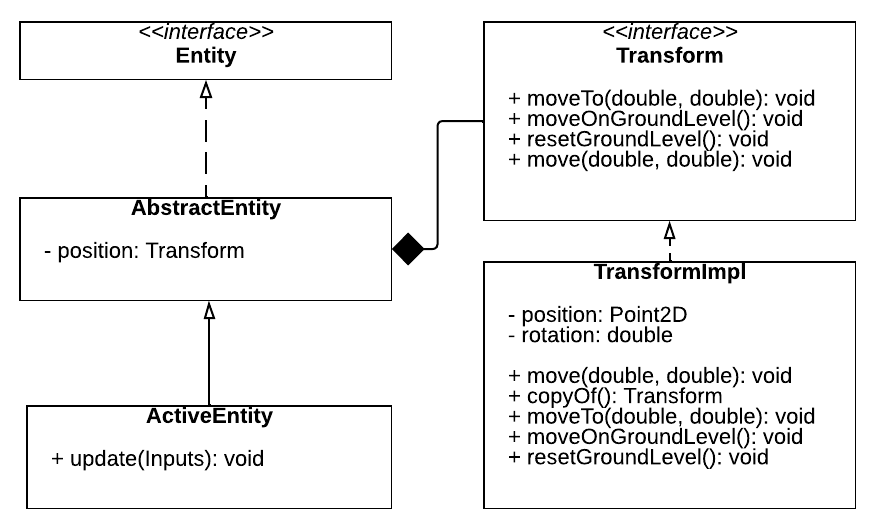
\includegraphics[width=1\textwidth]{images/Transform.png}
\caption{Integrazione del Transform}
\label{fig:transform}
\end{figure}

Le entità che ereditano direttamente da AbstractEntity hanno una posizione statica, mentre quelle che ereditano da ActiveEntity hanno una funzione update che in base all'input che ricevono modificano la loro posizione attraverso alterazioni della velocità. Per gestire questi movimenti ho implementato le funzioni moveTo, che sposta l'entità in un punto specificato in input, e move, che invece sposta l'entità di un offset su X e su Y che viene passato in input.\\
Per gestire le cadute ho implementato anche moveOnGroundLevel che controlla che l'entità non si trovi sotto il livello del suolo e, in tal caso, la riporta allo zero del sistema di riferimento.\\

All'interno della classe AbstractEntity ho anche implementato il metodo update che modifica la posizione dell'entità in base all'input che riceve.
In particolare gli input {$LEFT$} e {$RIGHT$} applicano un'accelerazione su X all'entity, mentre per il salto applica direttamente una velocità positiva su Y. Per la gravità e la decelerazione su X ho usato l'input {$EMPTY$} che applica un'accelerazione negativa su entrambi gli assi.\\

\textbf{Gestione dell'Input}\\

Un altro dei miei compiti era la gestione dell'input che ho implementato nella classe innestata di Game InputManager che sfrutta gli eventi dell'Application di JavaFX.\\

Per puntare l'arma infatti sfrutta le coordinate dell'evento onMouseMoved e per sparare quelle di onMouseClicked della Scene corrente.\\
Per la gestione dell'input simultaneo con i tasti A, D e Spazio ho utilizzato dei Boolean che rimangono true fintanto che i tasti rimangono premuti. in questo modo nella funzione update del Game Loop questi verranno considerati simultaneamente dal Player.\\
\textbf{Data Manager}\\

Fra i miei compiti c'era anche la parte di serializzazione e deserializzazione dei dati e dei livelli. Come formato per la serializzazione abbiamo scelto JSON e abbiamo utilizzato la libreria GSON di Google, che è stata integrata nella classe DataManager e in nelle varie classi per la deserializzazione.

\begin{figure}[ht]
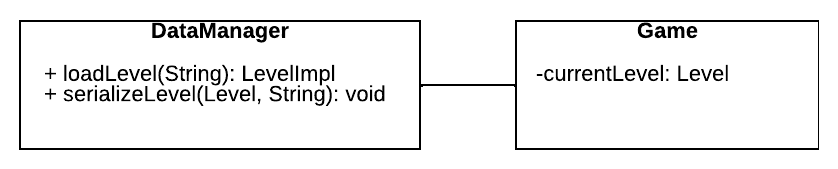
\includegraphics[width=1\textwidth]{images/DataManager.png}
\caption{Integrazione del DataManager}
\label{fig:datamanager}
\end{figure}

Il metodo serializeLevel, che prende in input un'istanza di Level e una stringa, genera un file json nominato come la stringa di input che conterrà i dati di tutte le Entity del livello e del Player. Questo metodo non è utilizzato nel software ma è risultato molto utile in fase di creazione dei livelli per poter creare agilmente i relativi json.\\
Il metodo loadLevel invece prende in input un file json precedentemente generato e ricostruisce il livello, tuttavia, per mantenere il file il più leggero possibile, non sono contenute diverse informazioni delle entità, pertanto le Entity deserializzate non sono complete ed è necessaria la funzione init per inizializzare alcuni componenti.

\subsection{Matteo Sartini}
\textbf{Bullet e Angle}\\
\\
Il mio task principale all’interno del progetto consisteva nell’ implementare un sistema che permettesse alle entità di sparare all’interno del livello in cui agiscono.
Per fare ciò in fase di progettazione, in linea con il modello ECS, abbiamo deciso di implementare un component Weapon, che permettesse alle entità che ne erano in possesso di creare nuove entità Bullet e dare loro una traiettoria verso cui muoversi.

\begin{figure}[ht]
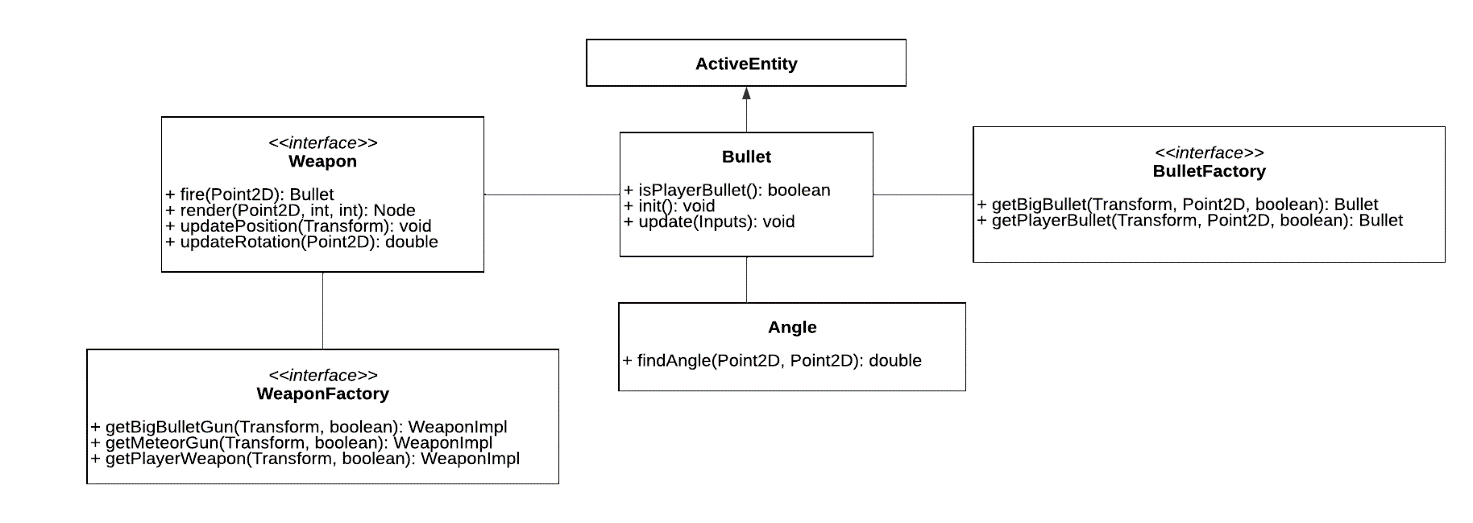
\includegraphics[width=1\textwidth]{images/UMLWeapon.png}
\caption{Metodi principali del component Weapon e dell’entità Bullet}
\label{fig:weapon}
\end{figure}

Richiamando il metodo fire viene restituita una nuova istanza dell’entità Bullet, creata attraverso l’utilizzo di una apposita Factory. A questa Entità Bullet vengono passate delle coordinate che rappresentano il punto mirato dalla entità (nel caso del player queste sono le coordinate del puntatore del mouse) che utilizza per estrapolare la traiettoria da mantenere per colpire il punto desiderato. Per fare questo ho ritenuto necessaria la scrittura di una classe utility Angle che mi permettesse di trovare l’angolo formato dal vettore teso tra due punti noti e il piano di riferimento del sistema. Il bullet una volta generato sarà gestito insieme alle altre entity del livello.
La classe Angle citata in precedenza è inoltre utilizzata per gestire la rotazione dell’arma del Player che è sempre orientata verso il puntatore del mouse.\\
\\
\textbf{Boss e Weapon}\\
\\
Weapon oltre alla sua funzione principale permette anche di essere renderizzato in sovrapposizione al suo user tramite un component Renderer.\\ La posizione di renderizzazione dell’arma e la posizione da cui vengono sparati i Bullet vengono aggiornate tramite un proprio component Transform durante l’update dell’entity a cui appartengono in base alla posizione di quest’ultima.

\begin{figure}[ht]
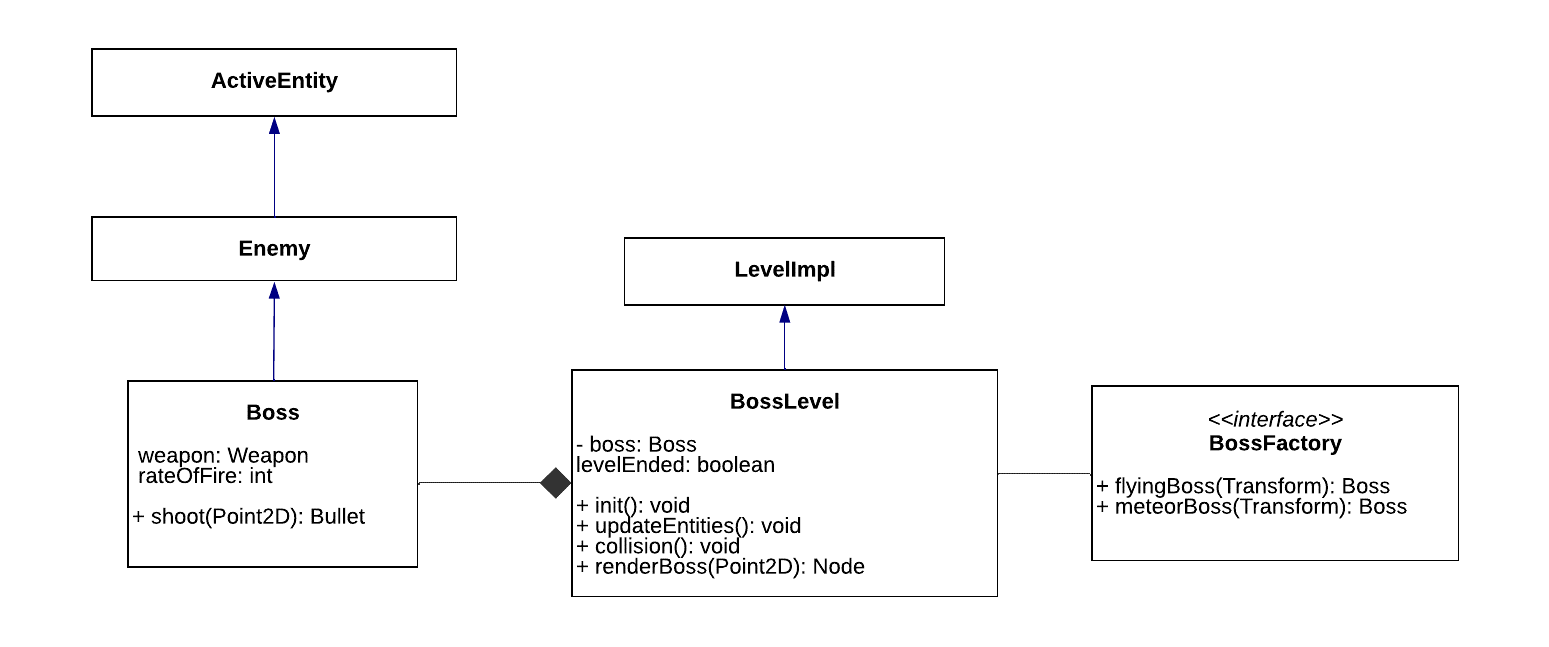
\includegraphics[width=1\textwidth]{images/UMLBoss.png}
\caption{Metodi per la gestione del Boss}
\label{fig:boss}
\end{figure}

In fase di progettazione abbiamo deciso di implementare le boss fight in apposite stanze e quindi in particolari livelli BossLevel. All’interno di questi livelli sono gestiti tutti i component del Boss come Weapon e Transform.
Il Boss vero e proprio è generato da una factory che mi ha permesso di personalizzare i diversi Boss a livello di funzionamento specifico, implementandone, ad esempio, uno capace di volare.
La classe Boss, estendendo Enemy, possiede tutti i suoi component e è capace di seguire dei Behaviour se inizializzati. Ciò che lo differenzia da un generico Enemy, oltre alla difficoltà incontrata nel combatterlo, è la presenza del component Weapon, che gli permettere di sparare.

\begin{figure}[ht]
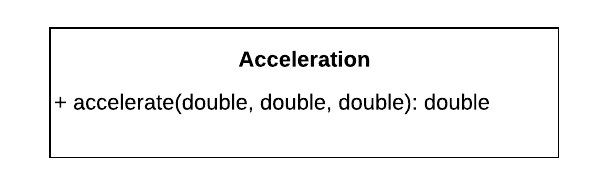
\includegraphics[width=1\textwidth]{images/UMLAcceleration.png}
\caption{Classe Acceleration}
\label{fig:acceleration}
\end{figure}

Infine ho implementato la classe di util Acceleration utilizzata nel movimento delle Entity per creare un effetto di movimento più fluido possibile.

\newpage
\chapter{Sviluppo}
\section{Testing automatizzato}
Sono state realizzate due classi di test, per valutare l'effettiva efficienza del gioco, implementate attraverso la libreria JUnit:
\begin{itemize}
\item TestEntity: controllo collisioni e danno
\item TestFinalGrade: controllo del corretto calcolo del punteggio finale
\end{itemize}
\section{Metodologie di lavoro}
Abbiamo iniziato lo sviluppo vero e proprio del software basandoci sulla fase di progettazione del design architetturale precedentemente effettuata. Inizialmente avevamo pensato ad una gerarchia di entità più articolata, rendendoci poi conto che questa contrastava con i principi del pattern architetturale da noi scelto; di conseguenza abbiamo dovuto effettuare delle modifiche in fase di integrazione, adeguando il design di partenza.
Per approcciarci alla realizzazione di questo progetto, abbiamo utilizzato il DVCS Git che ci ha permesso di coordinarne agevolmente lo sviluppo, integrando le varie parti con facilità. Abbiamo scelto di adottare una metodologia ispirata a GitFlow: il nostro branch principale è il 'master', nel quale abbiamo committato la versione corretta e funzionante del gioco; il branch di sviluppo di default è il 'develop' abbiamo creato inoltre dei branch dedicati allo sviluppo di particolari feature del gioco.
Vista la portata di lavoro del progetto, che nessuno di noi aveva mai affrontato in precedenza, abbiamo favorito il lavoro di gruppo e il confronto per la risoluzione dei problemi che si sono presentati.
\subsection{Livia Cardaccia}
Mi sono occupata dell'implementazione del component \texttt{Behaviour} e del \texttt{BehaviourBuilder}.
Ho creato i bottoni e le sub scenes del menu principale implementando le classi \texttt{CustumizedSubScene} e \texttt{CustomizedButton}, una finestra di dialogo personalizzata con la classe \texttt{ConfirmBox} e ho gestito il tutto con le classi \texttt{ViewManager} e \texttt{MainMenu}. Ho collaborato all'implementazione della classe \texttt{Score} con Denise Nanni e ho scritto la classe innestata\\ \texttt{SecondaryStage} in \texttt{Game}. Infine mi sono occupata delle entità rappresentanti gli ostacoli con le classi \texttt{Wall}, \texttt{Platform}, \texttt{HarmfulObstacle} e \texttt{Coin}.

\subsection{Denise Nanni}
Realizzazione della rilevazione e gestione delle collisioni in base alla direzione e calcolo di tale direzione.\\
\texttt{Logger} per mantenere uno storico degli errori verificatisi nell' applicativo.\\
Caricamento delle risorse attraverso reflection.\\
Realizzazione del calcolo del punteggio, insieme a Livia Cardaccia.\\

\subsection{Giovanni Prete}
I miei compiti principali all'interno del progetto sono stati\\
l'implementazione dei \texttt{Renderer} component, del \texttt{Transform} e della gestione dell'input. Mi sono occupato anche di alcuni metodi di \texttt{AbstractEntity}, \texttt{LevelImpl} e \texttt{Game} per la gestione delle classi che ho implementato. Infine mi sono dedicato alle meccaniche di serializzazione e deserializzazione, inoltre ho realizzato la classe utility \texttt{Window}, utilizzata come sistema di riferimento in diversi punti del codice.

\subsection{Matteo Sartini}
I task principali che mi sono stati assegnati all’interno del gruppo erano l’implementazione dell’arma e del suo funzionamento, compresi i suoi proiettili e l’implementazione, e la gestione all’interno di un apposito livello, del Boss. A questi elementi si sono andate ad aggiungere delle classi di supporto necessarie per la leggibilità del codice e alcuni elementi in classi esterne per l’implementazione dei vari elementi del codice tra loro.

\newpage
\section{Note di sviluppo}
\subsection{Livia Cardaccia}
\textbf{Utilizzo della libreria JavaFX}\\
Utilizzata per l'implementazione del menu di gioco. Un esempio è \href{https://github.com/dennnanni/UNIBOssfight/blob/61e1d141f734d2205d4e8b65fed0ebfc668a8357/UNIBOSSfight/src/main/java/app/ui/ViewManager.java#L31}{ViewManager}\\
\textbf{Utilizzo di lambda expressions}\\
Utilizzate in più punti del codice. Un esempio è la classe \href{https://github.com/dennnanni/UNIBOssfight/blob/61e1d141f734d2205d4e8b65fed0ebfc668a8357/UNIBOSSfight/src/main/java/app/impl/builder/BehaviourBuilderImpl.java#L13}{BehaviourBuilderImpl}\\
\textbf{Uso di Optional}\\
Utilizzati come tipo di ritorno dei metodi della classe
\href{https://github.com/dennnanni/UNIBOssfight/blob/61e1d141f734d2205d4e8b65fed0ebfc668a8357/UNIBOSSfight/src/main/java/app/impl/component/BehaviourImpl.java#L29}{BehaviourImpl}\\
\textbf{Programmazione funzionale}\\
\texttt{Biconsumer} e \texttt{Bifunction} utilizzati nell'implementazione del component Behaviour. Di seguito l'interfaccia \href{https://github.com/dennnanni/UNIBOssfight/blob/61e1d141f734d2205d4e8b65fed0ebfc668a8357/UNIBOSSfight/src/main/java/app/core/component/Behaviour.java#L14}{Behaviour}\\
\newline
Per capire il funzionamento della libreria JavaFX mi sono inizialmente affidata alla documentazione online; alcune parti di codice del menu di gioco, in particolare quelle relative alla creazione dei bottoni e l'implementazione dei listeners per ognuno di essi, sono riadattate da codice del seguente progetto \href{https://github.com/smowgli/space-runner-game-javafx/blob/dcbb51c278680951043d41d520e1a093f55701dc/src/model/SpaceRunnerButton.java#L11}{SpaceRunnerButton}.\\
Le grafiche del menu e i font li ho scaricati dal sito di \href{https://kenney.nl/}{Kenney}.\\
\subsection{Denise Nanni}
\textbf{Utilizzo di lambda expressions}
\newline
Utilizzate per valorizzare i comportamenti alla collisione. Un esempio è quello nella classe
\href{https://github.com/dennnanni/UNIBOssfight/blob/61e1d141f734d2205d4e8b65fed0ebfc668a8357/UNIBOSSfight/src/main/java/app/core/entity/Enemy.java#L34}{\underline{Enemy}}
\newline
\textbf{Utilizzo di Stream}
\newline
Utilizzati nella classe \href{https://github.com/dennnanni/UNIBOssfight/blob/61e1d141f734d2205d4e8b65fed0ebfc668a8357/UNIBOSSfight/src/main/java/app/game/Score.java#L60}{\underline{Score}}
\newline
\textbf{Logger}
\newline
Per lo sviluppo del logger ho consultato \href{https://www.digitalocean. com/community/tutorials/logger-in-java-logging-example}{\underline{questo link}}, oltre alla documentazione ufficiale.

\subsection{Giovanni Prete}
\textbf{Utilizzo di Stream}\\
Utilizzate in \href{https://github.com/dennnanni/UNIBOssfight/blob/0768464f3f7be0d1f35435f89616902091c0b7a8/UNIBOSSfight/src/main/java/app/impl/level/LevelImpl.java#L72}{updateEntities()} e \href{https://github.com/dennnanni/UNIBOssfight/blob/0768464f3f7be0d1f35435f89616902091c0b7a8/UNIBOSSfight/src/main/java/app/impl/level/LevelImpl.java#L125}{renderEntities()} di LevelImpl.\\
In \href{https://github.com/dennnanni/UNIBOssfight/blob/0b788e3202136a52ea940d4dedaac28589c7eb66/UNIBOSSfight/src/main/java/app/impl/component/LoopSpriteRenderer.java#L76}{initAnimation()} di \texttt{LoopSpriteRenderer}.

\textbf{Utilizzo di Gson}\\
In diverse classi util ma in particolare in \href{https://github.com/dennnanni/UNIBOssfight/blob/0b788e3202136a52ea940d4dedaac28589c7eb66/UNIBOSSfight/src/main/java/app/util/DataManager.java}{DataManager}

\textbf{Utilizzo di JavaFX}\\
In tutte le classi \texttt{Renderer} come ad esempio \href{https://github.com/dennnanni/UNIBOssfight/blob/0b788e3202136a52ea940d4dedaac28589c7eb66/UNIBOSSfight/src/main/java/app/impl/component/SpriteRenderer.java#L55}{SpriteRenderer}\\

Gli assets di gioco sono stati presi principalmente da pngegg.com e da craftpix.net

\subsection{Matteo Sartini}
\textbf{Utilizzo di lambda expressions}\\
Utilizzate in un metodo della classe \texttt{BehaviourBuilderImpl}
\href{https://github.com/dennnanni/UNIBOssfight/blob/1f248b375d7cf6e1bf10144a9acbacf9b59ca3b5/UNIBOSSfight/src/main/java/app/impl/builder/BehaviourBuilderImpl.java#L79}{metodo addFlying()}
\textbf{Utilizzo di Stream}\\
Utilizzati nella classe \href{https://github.com/dennnanni/UNIBOssfight/blob/1f248b375d7cf6e1bf10144a9acbacf9b59ca3b5/UNIBOSSfight/src/main/java/app/impl/level/BossLevel.java#L19}{BossLevel}


Inoltre per implementare le classe di utilità con più contenuto matematico ho utilizzato alcuni di tutorial della serie “Math for game developers” del canale YouTube “Jorge Rodriguez” che è possibile consultare a \href{https://www.youtube.com/playlist?list=PLW3Zl3wyJwWOpdhYedlD-yCB7WQoHf-My}{questo link}.

\large
\newpage
\chapter{Commenti finali}
\section{Autovalutazione e lavori futuri}
\subsection{Livia Cardaccia}
Dall'inizio del mio percorso universitario, questo è stato senza dubbio il lavoro più impegnativo: ha richiesto tempo e concentrazione ma soprattutto conoscenze che non avevo ancora completamente sviluppato durante il corso in aula ma che ho avuto l'occasione di approfondire durante la realizzazione del progetto. Lavorare in gruppo è stato un punto di forza, ci siamo confrontati e consigliati, il supporto che ci siamo dati l'un l'altro è stato secondo me fondamentale per la buona riuscita del progetto. Personalmente, una delle difficoltà più grandi che ho incontrato è stata scrivere codice pulito e soprattutto efficiente ma anche trovare soluzioni efficaci per i problemi presentatisi in itinere, affrontandoli riflettendo e analizzando le possibili soluzioni.\\
Come gruppo, una mancanza che secondo me abbiamo avuto è stata quella di non dedicare abbastanza tempo alla fase iniziale di analisi e progettazione: a posteriori posso dire che se ci fossimo soffermati di più su di essa, tutto il lavoro sarebbe risultato più fluido ed agevolato, quindi è sicuramente un aspetto che terrò a mente per eventuali progetti futuri.
Credo che questo percorso abbia permesso di migliorarmi sotto numerosi aspetti e che possa essere uno slancio per continuare a perfezionare le mie capacità; nel complesso, posso dire di essere soddisfatta del lavoro svolto.
\subsection{Denise Nanni}
Questo progetto ha rappresentato per me una grande sfida poiché, in molte occasioni, trovo difficile cimentarmi nei lavori di gruppo dato che preferisco rispettare i miei tempi e fare le cose a modo mio. Tuttavia, durante il percorso ci sono stati momenti in cui alcuni problemi riscontrati mi sembravano insormontabili e il sostegno dei miei compagni è stato di fondamentale importanza, perciò sono contenta di aver avuto un gruppo su cui contare.
Mi rendo conto di non essere stata molto collaborativa fin da subito, ma con l'inizio dello sviluppo vero e proprio credo di aver fatto il mio dovere e penso di essere stata d'aiuto per i miei compagni nel trovare soluzioni e idee, come loro lo sono stati per me.
Le più grandi difficoltà che ho riscontrato sono state la necessità di mantenere ben distinte le parti di mia competenza da quelle degli altri e il far fronte ai problemi che si sono presentati in itinere.\\
\subsection{Giovanni Prete}
Da quando ho iniziato a programmare alle superiori questa è stata la prima volta che posso dire di aver lavorato in un team e, nonostante sia stata l'esperienza più formativa finora, è stato difficile non avere tutto sotto controllo. Sento di essere stato spronato e di aver spronato a mia volta gli altri membri del team, rendendo piacevole il lavoro. Tuttavia, a posteriori, sento di aver fatto degli errori: in particolare una progettazione non troppo approfondita nelle fasi iniziali del progetto, che ha portato a codice difficile da scrivere e talvolta difficile da leggere. Nonostante alcune difficoltà, però, sono soddisfatto della gestione del game loop che rende il gioco abbastanza scorrevole.\\
\subsection{Matteo Sartini}
Nonostante le numerose difficoltà incontrate durante lo sviluppo, trovo che l’applicativo che ne è nato sia, con le sue numerose imperfezioni dovute alla poca esperienza del gruppo e alla complessità del progetto visualizzato in fase di progettazione, un prodotto abbastanza completo e per il quale mi ritengo molto soddisfatto.
Trovo però che la parte più stimolante del progetto sia stato il teamwork necessario al suo completamento. Ritengo infatti che la collaborazione tra i vari componenti di un team sia una skill assolutamente indispensabile nel nostro campo lavorativo, e troppo spesso ignorata in contesti scolastici.\\

\newpage
\chapter{Guida utente}
All'avvio del gioco si apre una schermata con il menu principale, in cui troviamo: un pulsante "play" per iniziare una nuova partita, un pulsante "level" per scegliere uno fra i due livelli proposti, un pulsante "help" per una breve spiegazione della modalità di gioco e un pulsante "score".
Cliccando quest'ultimo si possono visualizzare le proprie statistiche di gioco e una voce "final grade" che assegna al giocatore un punteggio in base alle sue prestazioni, nell'ottica del conseguimento della laurea.
Avviata una partita, per giocare è necessario: premere il tasto 'd' per correre in avanti, premere il tasto 'a' per correre indietro, usare la barra spaziatrice per saltare e il puntatore del mouse per mirare ai nemici, a cui si spara cliccando.
Terminata una partita vi è la possibilità di tornare alla home con un apposito pulsante o proseguire con il gioco.
\chapter{Esercitazioni di laboratorio}
\section{livia.cardaccia@studio.unibo.it}
\begin{itemize}
\item Laboratorio 03: \url{https://virtuale.unibo.it/mod/forum/discuss.php?d=112846\#p168413}
\item Laboratorio 05: \url{https://virtuale.unibo.it/mod/forum/discuss.php?d=114647\#p169868}
\item Laboratorio 06: \url{https://virtuale.unibo.it/mod/forum/discuss.php?d=115548\#p172236}
\item Laboratorio 07: \url{https://virtuale.unibo.it/mod/forum/discuss.php?d=117044\#p173315}
\item Laboratorio 08: \url{https://virtuale.unibo.it/mod/forum/discuss.php?d=117852\#p174528}
\item Laboratorio 09: \url{https://virtuale.unibo.it/mod/forum/discuss.php?d=118995\#p175251}
\item Laboratorio 10: \url{https://virtuale.unibo.it/mod/forum/discuss.php?d=119938\#p176896}
\item Laboratorio 11: \url{https://virtuale.unibo.it/mod/forum/discuss.php?d=121130\#p177745}
\end{itemize}
\section{denise.nanni@studio.unibo.it}
\begin{itemize}
\item Laboratorio 06: \url{https://virtuale.unibo.it/mod/forum/discuss.php?d=115548\#p171388}
\item Laboratorio 07: \url{https://virtuale.unibo.it/mod/forum/discuss.php?d=117044\#p173321}
\item Laboratorio 09: \url{https://virtuale.unibo.it/mod/forum/discuss.php?d=118995\#p175210}
\item Laboratorio 10: \url{https://virtuale.unibo.it/mod/forum/discuss.php?d=119938\#p176543}
\end{itemize}


\end{document}
